\documentclass[11pt,a4paper]{report}
\usepackage[textwidth=37em,vmargin=30mm]{geometry}
\usepackage{calc,xunicode,amsmath,amssymb,paralist,enumitem,tabu,booktabs,datetime2,xeCJK,xeCJKfntef,listings}
\usepackage{tocloft,fancyhdr,tcolorbox,xcolor,graphicx,eso-pic,xltxtra,xelatexemoji}

\newcommand{\envyear}[0]{2025}
\newcommand{\envdatestr}[0]{2025-05-22}
\newcommand{\envfinaldir}[0]{webdb/2025/20250522/final}

\usepackage[hidelinks]{hyperref}
\hypersetup{
    colorlinks=false,
    pdfpagemode=FullScreen,
    pdftitle={Web Digest - \envdatestr}
}

\setlength{\cftbeforechapskip}{10pt}
\renewcommand{\cftchapfont}{\rmfamily\bfseries\large\raggedright}
\setlength{\cftbeforesecskip}{2pt}
\renewcommand{\cftsecfont}{\sffamily\small\raggedright}

\setdefaultleftmargin{2em}{2em}{1em}{1em}{1em}{1em}

\usepackage{xeCJK,xeCJKfntef}
\xeCJKsetup{PunctStyle=plain,RubberPunctSkip=false,CJKglue=\strut\hskip 0pt plus 0.1em minus 0.05em,CJKecglue=\strut\hskip 0.22em plus 0.2em}
\XeTeXlinebreaklocale "zh"
\XeTeXlinebreakskip = 0pt


\setmainfont{Brygada 1918}
\setromanfont{Brygada 1918}
\setsansfont{IBM Plex Sans}
\setmonofont{JetBrains Mono NL}
\setCJKmainfont{Noto Serif CJK SC}
\setCJKromanfont{Noto Serif CJK SC}
\setCJKsansfont{Noto Sans CJK SC}
\setCJKmonofont{Noto Sans CJK SC}

\setlength{\parindent}{0pt}
\setlength{\parskip}{8pt}
\linespread{1.15}

\lstset{
	basicstyle=\ttfamily\footnotesize,
	numbersep=5pt,
	backgroundcolor=\color{black!5},
	showspaces=false,
	showstringspaces=false,
	showtabs=false,
	tabsize=2,
	captionpos=b,
	breaklines=true,
	breakatwhitespace=true,
	breakautoindent=true,
	linewidth=\textwidth
}






\newcommand{\coverpic}[2]{
    % argv: itemurl, authorname
    Cover photo by #2~~(\href{#1}{#1})
}
\newcommand{\makeheader}[0]{
    \begin{titlepage}
        % \newgeometry{hmargin=15mm,tmargin=21mm,bmargin=12mm}
        \begin{center}
            
            \rmfamily\scshape
            \fontspec{BaskervilleF}
            \fontspec{Old Standard}
            \fontsize{59pt}{70pt}\selectfont
            WEB\hfill DIGEST
            
            \vfill
            % \vskip 30pt
            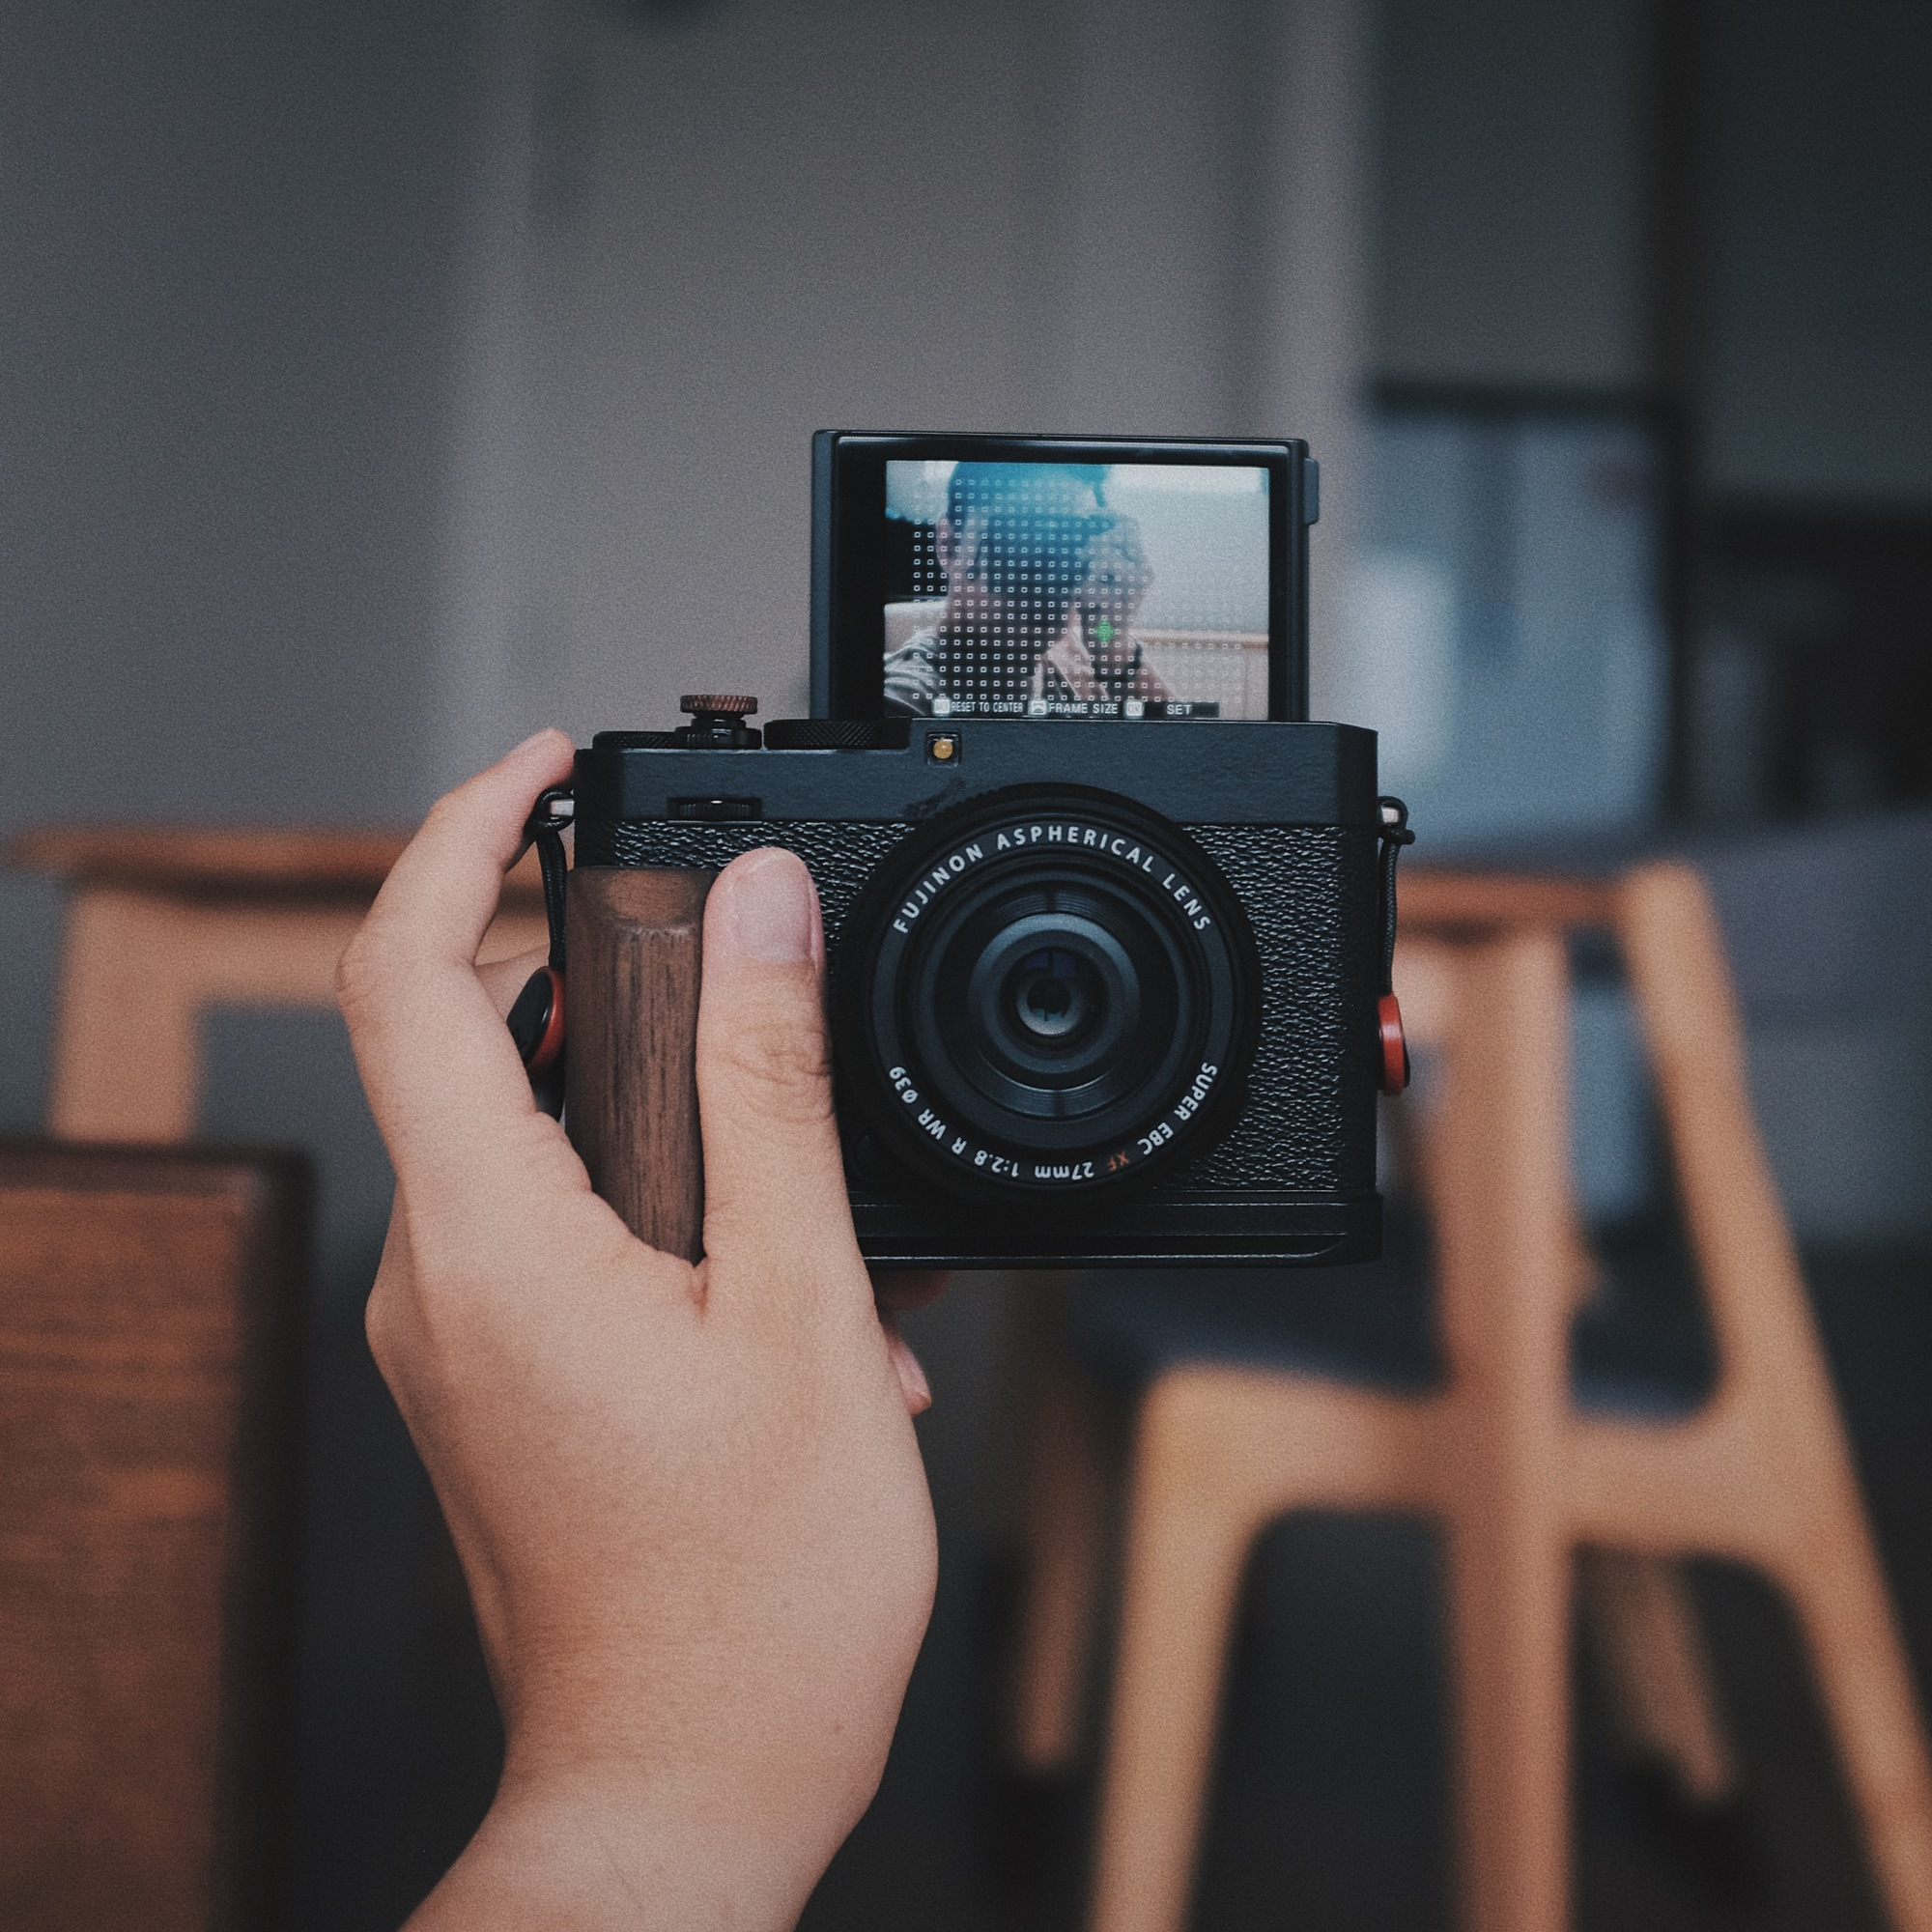
\includegraphics[width=\linewidth]{\envfinaldir/coverpic-prod.jpg}\par
            % \vskip 30pt
            \vfill

            \normalsize\rmfamily\scshape
            \copyright{} The Web Digest Project \hfill\large \envdatestr
        \end{center}
    \end{titlepage}
    % \restoregeometry
}
\newcommand{\simplehref}[1]{%
    \textcolor{blue!80!green}{\href{#1}{#1}}%
}
\renewcommand{\contentsname}{\center\Huge\sffamily\bfseries Contents\par\vskip 20pt}
\newcounter{ipartcounter}
\setcounter{ipartcounter}{0}
\newcommand{\ipart}[1]{
    % \vskip 20pt
    \clearpage
    \stepcounter{ipartcounter}
    \phantomsection
    \addcontentsline{toc}{chapter}{#1}
    % \begin{center}
    %     \Huge
    %     \sffamily\bfseries
    %     #1
    % \end{center}
    % \vskip 20pt plus 7pt
}
\newcounter{ichaptercounter}
\setcounter{ichaptercounter}{0}
\newcommand{\ichapter}[1]{
    % \vskip 20pt
    \clearpage
    \stepcounter{ichaptercounter}
    \phantomsection
    \addcontentsline{toc}{section}{\numberline{\arabic{ichaptercounter}}#1}
    \begin{center}
        \Huge
        \sffamily\bfseries
        #1
    \end{center}
    \vskip 20pt plus 7pt
}
\newcommand{\entrytitlefont}[1]{\subsection*{\raggedright\Large\sffamily\bfseries#1}}
\newcommand{\entryitemGeneric}[2]{
    % argv: title, url
    \parbox{\linewidth}{
        \entrytitlefont{#1}\par\vskip 5pt
        \footnotesize\ttfamily\mdseries
        \simplehref{#2}
    }\vskip 11pt plus 11pt minus 1pt
}
\newcommand{\entryitemGithub}[3]{
    % argv: title, url, desc
    \parbox{\linewidth}{
        \entrytitlefont{#1}\par\vskip 5pt
        \footnotesize\ttfamily\mdseries
        \simplehref{#2}\par\vskip 5pt
        \small\rmfamily\mdseries#3
    }\vskip 11pt plus 11pt minus 1pt
}
\newcommand{\entryitemAp}[3]{
    % argv: title, url, desc
    \parbox{\linewidth}{
        \entrytitlefont{#1}\par\vskip 5pt
        \footnotesize\ttfamily\mdseries
        \simplehref{#2}\par\vskip 5pt
        \small\rmfamily\mdseries#3
    }\vskip 11pt plus 11pt minus 1pt
}
\newcommand{\entryitemHackernews}[3]{
    % argv: title, hnurl, rawurl
    % \parbox{\linewidth}{
    %     \entrytitlefont{#1}\par\vskip 5pt
    %     \footnotesize\ttfamily\mdseries
    %     \simplehref{#3}\par
    %     \textcolor{black!50}{\href{#2}{#2}}
    % }\vskip 11pt plus 11pt minus 1pt
    \begin{minipage}{\linewidth}
            \entrytitlefont{#1}\par\vskip 5pt
            \footnotesize\ttfamily\mdseries
            \simplehref{#3}\par
            \textcolor{black!50}{\href{#2}{#2}}
    \end{minipage}\par\vskip 11pt plus 11pt minus 1pt
}







\begin{document}

\makeheader

\tableofcontents\clearpage




\ipart{Developers}
\ichapter{Hacker News}
\entryitemTwoLinks{For algorithms, a little memory outweighs a lot of time}{https://news.ycombinator.com/item?id=44055347}{https://www.quantamagazine.org/for-algorithms-a-little-memory-outweighs-a-lot-of-time-20250521/}

\entryitemTwoLinks{LLM function calls don't scale; code orchestration is simpler, more effective}{https://news.ycombinator.com/item?id=44053744}{https://jngiam.bearblog.dev/mcp-large-data/}

\entryitemTwoLinks{Storefront Web Components}{https://news.ycombinator.com/item?id=44053603}{https://shopify.dev/docs/api/storefront-web-components}

\entryitemTwoLinks{Collaborative Text Editing Without CRDTs or OT}{https://news.ycombinator.com/item?id=44053560}{https://mattweidner.com/2025/05/21/text-without-crdts.html}

\entryitemTwoLinks{OpenAI to buy AI startup from Jony Ive}{https://news.ycombinator.com/item?id=44053518}{https://www.bloomberg.com/news/articles/2025-05-21/openai-to-buy-apple-veteran-jony-ive-s-ai-device-startup-in-6-5-billion-deal}

\entryitemTwoLinks{By default, Signal doesn't recall}{https://news.ycombinator.com/item?id=44053364}{https://signal.org/blog/signal-doesnt-recall/}

\entryitemTwoLinks{Introducing the Llama Startup Program}{https://news.ycombinator.com/item?id=44052984}{https://ai.meta.com/blog/llama-startup-program/?\_fb\_noscript=1}

\entryitemTwoLinks{Discord Unveiled: A Comprehensive Dataset of Public Communication (2015-2024)}{https://news.ycombinator.com/item?id=44052041}{https://arxiv.org/abs/2502.00627}

\entryitemTwoLinks{Animated Factorization (2012)}{https://news.ycombinator.com/item?id=44051958}{http://www.datapointed.net/visualizations/math/factorization/animated-diagrams/}

\entryitemTwoLinks{Devstral}{https://news.ycombinator.com/item?id=44051733}{https://mistral.ai/news/devstral}

\entryitemTwoLinks{Things that have a bigger impact than coding assistants}{https://news.ycombinator.com/item?id=44050843}{https://codemanship.wordpress.com/2025/05/21/five-boring-things-that-have-a-bigger-impact-than-a-i-coding-assistants-on-dev-team-productivity/}

\entryitemTwoLinks{Roto: A Compiled Scripting Language for Rust}{https://news.ycombinator.com/item?id=44050222}{https://blog.nlnetlabs.nl/introducing-roto-a-compiled-scripting-language-for-rust/}

\entryitemTwoLinks{Watching AI drive Microsoft employees insane}{https://news.ycombinator.com/item?id=44050152}{https://old.reddit.com/r/ExperiencedDevs/comments/1krttqo/my\_new\_hobby\_watching\_ai\_slowly\_drive\_microsoft/}

\entryitemTwoLinks{The value isn't in the code (2022)}{https://news.ycombinator.com/item?id=44046955}{https://jonayre.uk/blog/2022/10/30/the-real-value-isnt-in-the-code/}

\entryitemTwoLinks{``ZLinq'', a Zero-Allocation LINQ Library for .NET}{https://news.ycombinator.com/item?id=44046578}{https://neuecc.medium.com/zlinq-a-zero-allocation-linq-library-for-net-1bb0a3e5c749}

\entryitemTwoLinks{Instagram Addiction}{https://news.ycombinator.com/item?id=44046559}{https://blog.greg.technology/2025/05/19/on-instagram-addiction.html}

\entryitemTwoLinks{Semantic search engine for ArXiv, biorxiv and medrxiv}{https://news.ycombinator.com/item?id=44046277}{https://arxivxplorer.com/}

\entryitemTwoLinks{Litestream: Revamped}{https://news.ycombinator.com/item?id=44045292}{https://fly.io/blog/litestream-revamped/}

\entryitemTwoLinks{The NSA Selector}{https://news.ycombinator.com/item?id=44044459}{https://github.com/wenzellabs/the\_NSA\_selector}

\entryitemTwoLinks{Gemma 3n preview: Mobile-first AI}{https://news.ycombinator.com/item?id=44044451}{https://developers.googleblog.com/en/introducing-gemma-3n/}\ichapter{Phoronix}
\entryitemGeneric{\hskip 0pt{}AMD Releases ROCm 6.4.1 With RDNA4 GPU Support}{https://www.phoronix.com/news/AMD-ROCm-6.4.1-Released}

\entryitemGeneric{\hskip 0pt{}libinput Preparing To Introduce A Lua-Based Plugin System For Modifying Devices/Events}{https://www.phoronix.com/news/libinput-Lua-Plugin-System}

\entryitemGeneric{\hskip 0pt{}Linux Improvements Boost AMD Ryzen Threadripper 7000 Series Performance Since Launch}{https://www.phoronix.com/review/amd-threadripper-7000-2025}

\entryitemGeneric{\hskip 0pt{}Fwupd 2.0.10 Brings Support For New Logitech \& Lenovo Devices}{https://www.phoronix.com/news/Fwupd-2.0.10-Released}

\entryitemGeneric{\hskip 0pt{}AMD To Focus On Better ROCm Linux Experience In H2-2025, Day-One Client Support}{https://www.phoronix.com/news/AMD-ROCm-H2-2025}

\entryitemGeneric{\hskip 0pt{}NVIDIA Outlines Current Wayland Limitations \& Future Driver Plans}{https://www.phoronix.com/news/NVIDIA-R575-Wayland-Plans}

\entryitemGeneric{\hskip 0pt{}FreeBSD Continues Improving Hardware Support For Framework Laptops, WiFi Devices}{https://www.phoronix.com/news/FreeBSD-Q1-2025}

\entryitemGeneric{\hskip 0pt{}Intel Compute Runtime 25.18.33578.6 Brings ULLS For Lunar Lake}{https://www.phoronix.com/news/Intel-CR-25.18.33578.6}

\entryitemGeneric{\hskip 0pt{}GNOME GDM Now Disables The X11/X.Org Session By Default}{https://www.phoronix.com/news/GNOME-GDM-Disable-X11-Default}\ichapter{Dribbble}
\entryitemGeneric{\hskip 0pt{}Illustration}{https://dribbble.com/shots/26052539-Illustration}

\entryitemGeneric{\hskip 0pt{}Playground web interaction}{https://dribbble.com/shots/26048246-Playground-web-interaction}

\entryitemGeneric{\hskip 0pt{}Travel Startup Branding for Holidu: visual identity brand design}{https://dribbble.com/shots/25983747-Travel-Startup-Branding-for-Holidu-visual-identity-brand-design}

\entryitemGeneric{\hskip 0pt{}DICH™ Fashion Vol.2}{https://dribbble.com/shots/26046875-DICH-Fashion-Vol-2}

\entryitemGeneric{\hskip 0pt{}L'Renee \& Associates logo}{https://dribbble.com/shots/26047943-L-Renee-Associates-logo}

\entryitemGeneric{\hskip 0pt{}Magus Logo Design}{https://dribbble.com/shots/26048055-Magus-Logo-Design}

\entryitemGeneric{\hskip 0pt{}Howdy from a happy hermit!}{https://dribbble.com/shots/26043217-Howdy-from-a-happy-hermit}

\entryitemGeneric{\hskip 0pt{}F}{https://dribbble.com/shots/26041370-F}

\entryitemGeneric{\hskip 0pt{}Mackerel}{https://dribbble.com/shots/26043994-Mackerel}

\entryitemGeneric{\hskip 0pt{}Evergreen}{https://dribbble.com/shots/26042187-Evergreen}

\entryitemGeneric{\hskip 0pt{}Dark or Light?}{https://dribbble.com/shots/26042325-Dark-or-Light}

\entryitemGeneric{\hskip 0pt{}Planto}{https://dribbble.com/shots/26044620-Planto}

\entryitemGeneric{\hskip 0pt{}QueenClub Logo Design}{https://dribbble.com/shots/26042947-QueenClub-Logo-Design}

\entryitemGeneric{\hskip 0pt{}Ebay Rebranding Concept}{https://dribbble.com/shots/26039712-Ebay-Rebranding-Concept}

\entryitemGeneric{\hskip 0pt{}Profile Card 👧}{https://dribbble.com/shots/26033069-Profile-Card}

\entryitemGeneric{\hskip 0pt{}DICH™ Fashion}{https://dribbble.com/shots/26032014-DICH-Fashion}

\entryitemGeneric{\hskip 0pt{}Techtots on UI8 illustration set}{https://dribbble.com/shots/25995896-Techtots-on-UI8-illustration-set}

\entryitemGeneric{\hskip 0pt{}East Meats West}{https://dribbble.com/shots/26027917-East-Meats-West}

\entryitemGeneric{\hskip 0pt{}Assist Logo Design (Unused for Sale)}{https://dribbble.com/shots/26027053-Assist-Logo-Design-Unused-for-Sale}

\entryitemGeneric{\hskip 0pt{}Goldfish Concept}{https://dribbble.com/shots/26029115-Goldfish-Concept}

\entryitemGeneric{\hskip 0pt{}Sellin dashboard}{https://dribbble.com/shots/26027518-Sellin-dashboard}

\entryitemGeneric{\hskip 0pt{}Matte Glass Logo}{https://dribbble.com/shots/26027999-Matte-Glass-Logo}

\entryitemGeneric{\hskip 0pt{}Healthcare Dashboard UI/UX Design}{https://dribbble.com/shots/26026655-Healthcare-Dashboard-UI-UX-Design}

\entryitemGeneric{\hskip 0pt{}Watch Face}{https://dribbble.com/shots/26030361-Watch-Face}


\ipart{Developers~~~~(zh-Hans)}
\ichapter{Solidot}
\entryitemGeneric{\hskip 0pt{}猴痘全球疫情爆发前已在尼日利亚传播了八年}{https://www.solidot.org/story?sid=81354}

\entryitemGeneric{\hskip 0pt{}俄罗斯停止公开人口统计数据细节}{https://www.solidot.org/story?sid=81353}

\entryitemGeneric{\hskip 0pt{}IEEE 刊登的一篇论文被发现包含中文脏话}{https://www.solidot.org/story?sid=81352}

\entryitemGeneric{\hskip 0pt{}法国禁止 Telegram 创始人 Pavel Durov 前往美国}{https://www.solidot.org/story?sid=81350}

\entryitemGeneric{\hskip 0pt{}报纸刊登的推荐书单名被发现多数是 AI 捏造的}{https://www.solidot.org/story?sid=81349}

\entryitemGeneric{\hskip 0pt{}美国大学城走向萧条}{https://www.solidot.org/story?sid=81348}

\entryitemGeneric{\hskip 0pt{}Google 搜索开始向美国用户提供 AI 模式}{https://www.solidot.org/story?sid=81347}

\entryitemGeneric{\hskip 0pt{}微软封了国际刑事法院首席检察官的电邮账号}{https://www.solidot.org/story?sid=81346}

\entryitemGeneric{\hskip 0pt{}调查发现气候科学家是最不受信任的科学家}{https://www.solidot.org/story?sid=81345}

\entryitemGeneric{\hskip 0pt{}Red Hat 宣布 RHEL 10,推出针对 RISC-V 架构的开发者预览版}{https://www.solidot.org/story?sid=81344}

\entryitemGeneric{\hskip 0pt{}4 月中国智能手机出口暴跌 72\%}{https://www.solidot.org/story?sid=81343}

\entryitemGeneric{\hskip 0pt{}丹麦考虑建造核电}{https://www.solidot.org/story?sid=81342}

\entryitemGeneric{\hskip 0pt{}2024 年电动汽车占到汽车总销量逾五分之一}{https://www.solidot.org/story?sid=81341}

\entryitemGeneric{\hskip 0pt{}超加工食品微塑料在人脑积累可能会引起心理健康问题}{https://www.solidot.org/story?sid=81340}

\entryitemGeneric{\hskip 0pt{}人体肺活量衰减始于 20-25 岁}{https://www.solidot.org/story?sid=81339}

\entryitemGeneric{\hskip 0pt{}7-Eleven 在东京都地区测试机器人送货}{https://www.solidot.org/story?sid=81338}

\entryitemGeneric{\hskip 0pt{}分数量子反常霍尔效应}{https://www.solidot.org/story?sid=81337}

\entryitemGeneric{\hskip 0pt{}微软开源 Windows Subsystem for Linux}{https://www.solidot.org/story?sid=81336}

\entryitemGeneric{\hskip 0pt{}DDoSecrets 发布窃取自 TeleMessage 的 410 GB 数据集}{https://www.solidot.org/story?sid=81335}

\entryitemGeneric{\hskip 0pt{}Firefox 快速释出更新修复两个 Pwn2Own 上公开的漏洞利用}{https://www.solidot.org/story?sid=81334}\ichapter{V2EX}
\entryitemGeneric{\hskip 0pt{}[问与答] 还有那些类似 Samurai II: Vengeance 这种单机手游}{https://www.v2ex.com/t/1133402}

\entryitemGeneric{\hskip 0pt{}[分享创造] I2C/SPI 和元件通信的数据内容}{https://www.v2ex.com/t/1133401}

\entryitemGeneric{\hskip 0pt{}[云计算] 云原生有没有不错的实验课}{https://www.v2ex.com/t/1133400}

\entryitemGeneric{\hskip 0pt{}[旅行] 四月底去德国旅行小记}{https://www.v2ex.com/t/1133399}

\entryitemGeneric{\hskip 0pt{}[macOS] 各位, mac 的系统更新设置到底怎么设置最佳?}{https://www.v2ex.com/t/1133398}

\entryitemGeneric{\hskip 0pt{}[程序员] 想买个海外号码,长期接短信验证码用,有推荐吗?}{https://www.v2ex.com/t/1133396}

\entryitemGeneric{\hskip 0pt{}[生活] 让 Gpt 当了把心理医生}{https://www.v2ex.com/t/1133395}

\entryitemGeneric{\hskip 0pt{}[Bitcoin] 比特币又创历史新高了}{https://www.v2ex.com/t/1133394}

\entryitemGeneric{\hskip 0pt{}[问与答] 经常去香港购物的麻烦来帮我解答一下免税额度}{https://www.v2ex.com/t/1133392}

\entryitemGeneric{\hskip 0pt{}[程序员] 不得不感叹下 ChatGPT 的多模态太好用了!}{https://www.v2ex.com/t/1133391}

\entryitemGeneric{\hskip 0pt{}[Node.js] redis 集群模式支持批量操作库 mget/mset}{https://www.v2ex.com/t/1133390}

\entryitemGeneric{\hskip 0pt{}[宽带症候群] 单宽带到期后,再办理算是新办宽带吗?}{https://www.v2ex.com/t/1133389}

\entryitemGeneric{\hskip 0pt{}[设计] 做了一个给图片添加矢量描边的 Figma 插件}{https://www.v2ex.com/t/1133388}

\entryitemGeneric{\hskip 0pt{}[DNS] 梅林固件设置里的 dns-dot 最近好像不能用了}{https://www.v2ex.com/t/1133387}

\entryitemGeneric{\hskip 0pt{}[职场话题] 同样是发 offer,为什么不同的企业完全不一样}{https://www.v2ex.com/t/1133385}

\entryitemGeneric{\hskip 0pt{}[远程工作] [全职远程工作 ] 下一代桌面级编辑器 Lattics 前端开发(限 1 ~ 5 年工作经验)}{https://www.v2ex.com/t/1133383}

\entryitemGeneric{\hskip 0pt{}[路由器] opnsense 网络配置问题,头快抓破了}{https://www.v2ex.com/t/1133382}

\entryitemGeneric{\hskip 0pt{}[问与答] 用 openwrt 做旁路由,访问某些网址会显示证书不安全,点击继续访问网址会自动添加/cgi-bin/luci/这串后缀,然后自动进入旁路由后台,是什么原因啊}{https://www.v2ex.com/t/1133381}

\entryitemGeneric{\hskip 0pt{}[分享发现] 我好像一直是个纠结的人,不知道能不能慢慢改一点}{https://www.v2ex.com/t/1133380}

\entryitemGeneric{\hskip 0pt{}[SSL] [求助]在阿里云 ECS Nginx 安装 godaddy SSL 证书后, Windows 的浏览器可以访问, iOS/MacOS 的浏览器打不开}{https://www.v2ex.com/t/1133379}

\entryitemGeneric{\hskip 0pt{}[硬件] 求推荐一款影音平板}{https://www.v2ex.com/t/1133378}

\entryitemGeneric{\hskip 0pt{}[问与答] 一款几十万人常用的 App 有多赚钱?}{https://www.v2ex.com/t/1133377}

\entryitemGeneric{\hskip 0pt{}[分享创造] http-stat-rs:纯 rust 实现的类 curl 工具}{https://www.v2ex.com/t/1133376}

\entryitemGeneric{\hskip 0pt{}[职场话题] 在北京程序员能干什么和写代码无关的兼职呢}{https://www.v2ex.com/t/1133375}

\entryitemGeneric{\hskip 0pt{}[分享创造] 做了一个八字推演的网站,}{https://www.v2ex.com/t/1133374}

\entryitemGeneric{\hskip 0pt{}[App Store] Mac App Store 无法安装新 APP}{https://www.v2ex.com/t/1133373}

\entryitemGeneric{\hskip 0pt{}[问与答] 请问类似 https://roadmap.sh/的路线图的 JS 库或开源软件有那些}{https://www.v2ex.com/t/1133372}

\entryitemGeneric{\hskip 0pt{}[职场话题] 分享下工作中遇到的趣事}{https://www.v2ex.com/t/1133370}

\entryitemGeneric{\hskip 0pt{}[问与答] 最近买了一个 bose qc45 降噪耳机,开降噪头晕恶心、开通透风噪呼呼的,人都麻了,问了客服也不能退。}{https://www.v2ex.com/t/1133369}

\entryitemGeneric{\hskip 0pt{}[问与答] 如何提升学历?}{https://www.v2ex.com/t/1133368}

\entryitemGeneric{\hskip 0pt{}[程序员] 调研一下大家解析 Markdown 都用过什么库}{https://www.v2ex.com/t/1133367}

\entryitemGeneric{\hskip 0pt{}[电影] 年龄大了 ,看到破地狱这样的电影反而有不一样的感受}{https://www.v2ex.com/t/1133365}

\entryitemGeneric{\hskip 0pt{}[程序员] 有办法获取多多的直播链接和直播回放链接么?}{https://www.v2ex.com/t/1133364}

\entryitemGeneric{\hskip 0pt{}[MacBook Pro] 各位有用 M4 Pro MacBook Pro 搞开发的吗?日常使用烫不烫?}{https://www.v2ex.com/t/1133362}

\entryitemGeneric{\hskip 0pt{}[问与答] KDE wayland 环境下 Electron 的 appimage 程序没有边框和阴影}{https://www.v2ex.com/t/1133361}

\entryitemGeneric{\hskip 0pt{}[投资] 30+的投资者加个圈子}{https://www.v2ex.com/t/1133360}

\entryitemGeneric{\hskip 0pt{}[问与答] 前端有没有轻量级的流程图工具求推荐}{https://www.v2ex.com/t/1133359}

\entryitemGeneric{\hskip 0pt{}[生活] 我们都在用力的活着}{https://www.v2ex.com/t/1133358}

\entryitemGeneric{\hskip 0pt{}[酷工作] [懂车帝] [北京/杭州/重庆] 招初级前端工程狮}{https://www.v2ex.com/t/1133357}

\entryitemGeneric{\hskip 0pt{}[硬件] 小米 15spro 提前泄漏:玄戒跑分略胜骁龙 8E,电池容量变大}{https://www.v2ex.com/t/1133355}

\entryitemGeneric{\hskip 0pt{}[宽带症候群] 广东电信联通省内跨网不癫了?}{https://www.v2ex.com/t/1133354}

\entryitemGeneric{\hskip 0pt{}[分享创造] 免费的 CDN 防盗刷解决方案,彻底杜绝 CDN 流量被盗刷}{https://www.v2ex.com/t/1133353}

\entryitemGeneric{\hskip 0pt{}[问与答] 电信骚扰短信求解决办法!}{https://www.v2ex.com/t/1133352}

\entryitemGeneric{\hskip 0pt{}[问与答] android studio 总是弹出让我输入认证账号密码}{https://www.v2ex.com/t/1133350}

\entryitemGeneric{\hskip 0pt{}[NAS] 老硬盘还真不能用}{https://www.v2ex.com/t/1133349}

\entryitemGeneric{\hskip 0pt{}[问与答] 2025 了,现在 CPU 还能买散片吗?}{https://www.v2ex.com/t/1133348}

\entryitemGeneric{\hskip 0pt{}[生活] 这里面有什么隐情吗?}{https://www.v2ex.com/t/1133346}

\entryitemGeneric{\hskip 0pt{}[酷工作] [ios 开发] 出海短视频社交项目}{https://www.v2ex.com/t/1133345}

\entryitemGeneric{\hskip 0pt{}[硬件] 微星 B550M 迫击炮 wifi 主板, BIOS 固件最近版本,两个 M.2 固态都会掉盘是什么问题?主板坏了吗?}{https://www.v2ex.com/t/1133344}

\entryitemGeneric{\hskip 0pt{}[问与答] 阿里云 CDN 请求费现在一个月 2000 钱多...换哪家求推荐}{https://www.v2ex.com/t/1133343}


\ipart{Generic News}
\ichapter{AP News}
\entryitemWithDescription{\hskip 0pt{}Former New York state trooper pleads guilty to faking his own shooting}{https://apnews.com/article/5b822d3e3da0d51978637fff6eb6e2ff}{}

\entryitemWithDescription{\hskip 0pt{}UK court frees singer Chris Brown freed on \$6.7 million bail in assault case}{https://apnews.com/article/6d4ae244ea7729609a34cc7825733a70}{}

\entryitemWithDescription{\hskip 0pt{}George Wendt, who played beloved barfly Norm on `Cheers' and found another home onstage, dies at 76}{https://apnews.com/article/55681263ea8b5bddaf1c89e8e9ba8cb1}{}

\entryitemWithDescription{\hskip 0pt{}Southwest Airlines will require chargers be kept out while in use because of battery fire concerns}{https://apnews.com/article/736e74e55a6467b0b12e3938653de169}{}

\entryitemWithDescription{\hskip 0pt{}On `World Bee Day,' the bees did not seem bothered. They should be}{https://apnews.com/article/498d981856e9963235c02cac11160c9e}{}

\entryitemWithDescription{\hskip 0pt{}Levi Strauss agrees to sell Casual Friday staple Dockers for up to \$391 million}{https://apnews.com/article/2738cb9f4f1fa52443cf54ff752db5b7}{}

\entryitemWithDescription{\hskip 0pt{}Home Depot says it doesn't expect to boost prices because of tariffs}{https://apnews.com/article/47e51f7c5c18a5e5a7f407fd25269430}{}

\entryitemWithDescription{\hskip 0pt{}Passenger jet had to abort takeoff to avoid runway collision at New York's LaGuardia Airport}{https://apnews.com/article/821fcc0a18d5da17b832b2e17af765c0}{}

\entryitemWithDescription{\hskip 0pt{}Trump administration agrees to pay nearly \$5M to settle suit over Ashli Babbitt shooting in Capitol}{https://apnews.com/article/6de2a507ddac903c68c5d3a25f35f24c}{}

\entryitemWithDescription{\hskip 0pt{}Austria welcomes JJ back home with cheers, hugs and roses after he wins the Eurovision Song Contest}{https://apnews.com/article/1172835ced038ec1efa197fca39fbf5c}{}

\entryitemWithDescription{\hskip 0pt{}Missing hiker survived for weeks in California wilderness by foraging and drinking melted snow}{https://apnews.com/article/9ede4b951c577c96d0fed3915b257cfd}{}

\entryitemWithDescription{\hskip 0pt{}Former MLB star Rafael Furcal charged in rock-throwing road rage incident, police say}{https://apnews.com/article/84d45518fa54d06605e4aef865844916}{}

\entryitemWithDescription{\hskip 0pt{}Former President George W. Bush draws inspiration close to his Dallas home in his latest paintings}{https://apnews.com/article/38c9e923ec84bd2b3c55be21a2d1f100}{}\ichapter{Reuters}
\entryitemWithDescription{\hskip 0pt{}Exclusive: US Army to change transgender soldiers' records to birth sex}{https://www.reuters.com/world/us/us-army-change-transgender-soldiers-records-birth-sex-2025-05-21/}{The U.S. Army will alter the records of transgender soldiers to show only their sex at birth, according to internal guidance seen by Reuters that details a series of steps it will take as it pushes them out of the...}

\entryitemWithDescription{\hskip 0pt{}Kosovo's political stalemate could put EU funds at risk, trade body warns}{https://www.reuters.com/world/kosovos-political-stalemate-could-put-eu-funds-risk-trade-body-warns-2025-05-21/}{Kosovo\textquotesingle s parliament failed to elect a new speaker for the 15th straight time on Wednesday, prompting fears of an economic backlash after months of political stalemate in one of Europe's poorest...}

\entryitemWithDescription{\hskip 0pt{}Israel Supreme Court says decision to sack Shin Bet chief was illegal, Israeli media report}{https://www.reuters.com/world/middle-east/israels-supreme-court-rules-that-decision-sack-shin-bet-chief-was-illegal-2025-05-21/}{Israel\textquotesingle s Supreme Court has ruled that a government decision to sack the head of the domestic intelligence service Shin Bet was "illegal and contrary to law", Israeli media reported on...}

\entryitemWithDescription{\hskip 0pt{}Portugal to investigate far-right leader over anti-Roma remarks}{https://www.reuters.com/business/media-telecom/portugal-investigate-far-right-leader-over-anti-roma-remarks-2025-05-21/}{Portuguese prosecutors have opened a probe into remarks made by far-right leader Andre Ventura against the Roma community, three days after an election in which his Chega party surged and was tied for second place in...}

\entryitemWithDescription{\hskip 0pt{}UK anti-Islam activist 'Tommy Robinson' charged with harassment of two men}{https://www.reuters.com/world/uk/uk-anti-islam-activist-tommy-robinson-charged-with-harassment-two-men-2025-05-21/}{Prominent British anti-Islam activist Stephen Yaxley-Lennon has been charged with harassment causing fear of violence to two men around the time of the nationwide riots last year, prosecutors said on...}

\entryitemWithDescription{\hskip 0pt{}US aims to deport 8 serious criminals, Trump official says, won't confirm South Sudan destination}{https://www.reuters.com/world/us/trump-official-says-us-seeking-deport-eight-serious-criminals-declines-confirm-2025-05-21/}{A Homeland Security official said on Wednesday that the U.S. is seeking to deport eight migrants convicted of serious crimes including homicides, but declined to confirm an allegation raised in federal court that they were bound for South...}

\entryitemWithDescription{\hskip 0pt{}Israeli soldiers fire near diplomats on visit to occupied West Bank}{https://www.reuters.com/world/europe/israeli-soldiers-fire-near-diplomats-visit-occupied-west-bank-2025-05-21/}{The Israeli military said that it fired near a diplomatic delegation which it said deviated from an approved route in the occupied West Bank on...}

\entryitemWithDescription{\hskip 0pt{}Russia says it downed over 232 Ukrainian drones, forcing Moscow airports to halt some flights}{https://www.reuters.com/world/europe/russia-says-it-downed-over-232-ukrainian-drones-forcing-moscow-airports-halt-2025-05-21/}{Russia said on Wednesday that its air defences had shot down at least 232 Ukrainian drones over various Russian regions, including some approaching Moscow where the capital\textquotesingle s airports were briefly shut down to ensure the...}

\entryitemWithDescription{\hskip 0pt{}EU envoys reach deal on 150 billion euro arms fund}{https://www.reuters.com/business/aerospace-defense/eu-envoys-reach-deal-150-billion-euro-arms-fund-2025-05-21/}{European Union ambassadors signed off on Wednesday on a new flagship arms-buying fund, being set up quickly to provide 150 billion euros (\$170 billion) in loans for defence projects, driven by fears of Russia and doubts about future U.S...}

\entryitemWithDescription{\hskip 0pt{}UK and allies warn of Russian cyber activity targeting support to Ukraine}{https://www.reuters.com/world/uk-allies-warn-russian-cyber-activity-targeting-support-ukraine-2025-05-21/}{Britain and allies including the United States issued an advisory on Wednesday warning of a Russian state-sponsored cyber campaign targeting the delivery of support to Ukraine and Western logistics entities and technology...}

\entryitemWithDescription{\hskip 0pt{}Finland completes first 35 km of fence on Russian border}{https://www.reuters.com/world/finland-completes-first-35-km-fence-russian-border-2025-05-21/}{Finland has completed the first 35 km (22 miles) of a 4.5-metre (15-ft) high fence it is building on its closed eastern border with Russia to stop migrants from crossing via the wilderness, the Finnish Border Guard said on...}

\entryitemWithDescription{\hskip 0pt{}UK pledges over \$5 million in aid to Gaza}{https://www.reuters.com/world/uk/uk-pledges-over-5-million-humanitarian-aid-gaza-2025-05-21/}{Britain pledged 4 million pounds (\$5.4 million) in humanitarian aid to Gaza, the government said on Wednesday, as its Minister for Development Jenny Chapman visited Israel and the occupied Palestinian...}

\entryitemWithDescription{\hskip 0pt{}Gaza still waiting for aid as pressure mounts on Israel}{https://www.reuters.com/world/middle-east/gaza-still-waiting-aid-pressure-mounts-israel-2025-05-21/}{No aid has reached people in Gaza, a U.N. aid official said on Wednesday, two days after the Israeli government said it had lifted an 11-week-old blockade that has brought the Palestinian enclave to the brink of...}






\clearpage
\leavevmode\vfill
\footnotesize

Copyright \copyright{} 2023-2025 Neruthes and other contributors.

This document is published with CC BY-NC-ND 4.0 license.

The entries listed in this newsletter may be copyrighted by their respective creators.

This newsletter is generated by the Web Digest project.

The newsletters are also delivered via Telegram channel \CJKunderline{\href{https://t.me/webdigestchannel}{https://t.me/webdigestchannel}}.\\
RSS feed is available at \CJKunderline{\href{https://webdigest.pages.dev/rss.xml}{https://webdigest.pages.dev/rss.xml}}.

This newsletter is available in PDF at
\CJKunderline{\href{https://webdigest.pages.dev/}{https://webdigest.pages.dev/}}.

The source code being used to generate this newsletter is available at\\
\CJKunderline{\href{https://github.com/neruthes/webdigest}{https://github.com/neruthes/webdigest}}.

This newsletter is also available in
\CJKunderline{\href{http://webdigest.pages.dev/readhtml/\envyear/WebDigest-20250522.html}{HTML}} and
\CJKunderline{\href{https://github.com/neruthes/webdigest/blob/master/markdown/\envyear/WebDigest-20250522.md}{Markdown}}.


\coverpic{https://unsplash.com/photos/people-line-up-at-a-japanese-food-stall-7c524C8mN7g}{HANVIN CHEONG}


\end{document}
